\documentclass[10pt,oneside,openright]{report} 

\title{Sequence to Sequence learning using Variational Information Bottleneck}
\author{Tristan Guigue}
\date{2017}

\usepackage[mastersc]{edmaths}
\usepackage[parfill]{parskip}
\usepackage[english]{babel}
\usepackage[utf8]{inputenc}
\usepackage{amsmath}
\usepackage{graphicx}
\usepackage[colorinlistoftodos]{todonotes}
\usepackage{amsmath,amsfonts,amssymb}
\usepackage{float}
\usepackage{tikz}
\usetikzlibrary{bayesnet}
\usetikzlibrary{fit, positioning, arrows.meta}
\usepackage[makeroom]{cancel}
\tikzset{
neuron/.style={shape=circle, minimum size=1.1cm,  inner sep=0, draw, font=\small}, io/.style={neuron, fill=gray!20}, deterministic/.style={diamond, minimum size=1.3cm, draw, text badly centered, inner sep=3pt}}
\newtheorem{notation}{Notation}
\newtheorem{definition}{Definition}
\newtheorem{corollary}{Corollary}
\newtheorem{theorem}{Theorem}
\newtheorem{lemma}{Lemma}

\begin{document}

\maketitle

\declaration

\begin{abstract}
TODO
\end{abstract}

\tableofcontents

%------------------------------------------------------------------------------------------------
\chapter{Introduction}
TODO
%------------------------------------------------------------------------------------------------
\chapter{Background and Literature Review}

\section{The Information Bottleneck}
\subsection{Regularisation in Supervised Learning}
In supervised learning, we try to infer an output: the random variable $Y$ from an input given by the random variable $X$, learning from labelled training data. The objective is to learn a mapping from $X$ to $Y$ that generalises well to unseen data. To avoid overfitting, that is to ensure the learning process learns the underlying relationship between $X$ and $Y$ rather than noise in the training data, there are different ways to regularise, promoting simpler mappings. We assume here there is indeed an underlying relationship between $X$ and $Y$ so $Y$ must not be independent from the input $X$.

One form of regularisation was introduced by Tishby et al. \cite{tishby}. For each input they seek a stochastic mapping to a representation of the input that provides the most relevant information about the output. They used information theory principles to formalise what a good representation of the input should be extracted. 

The objective is to learn a representation $Z$ that is maximally compressive on $X$ while being maximally informative about the target $Y$. We want to squeeze the information that $X$ contains about $Y$ trough a bottleneck and keep only the most meaningful information about the output. For example when learning the transcript of words from acoustic data, it is possible to greatly compress the input data while still keeping what is useful to predict the words.

\subsection{Mutual Information}

\begin{definition}
The amount of information that $Z$ contains about $Y$ is given by:
$$ I(Z, Y) = \int p(y, z) \log \frac{p(z, y)}{p(z)p(y)} dy\,dz $$ where Y and Z are continous random variables or 
 $$ I(Z, Y) = \sum_y \sum_z p(y, z) \log \frac{p(z, y)}{p(z)p(y)} $$ where Y and Z are discrete random variables 
\end{definition}

\begin{definition}
The KL divergence from a continuous probability distribution $p$ to another continuous probability distribution $q$ is defined as 
$$ KL[p(x)|q(x)] = \int p(x) \log \frac{p(x)}{q(x)} dx $$
\end{definition}

\begin{corollary}
The mutual information of two random variable is equal to the Kullback-Leibler divergence from the joint distribution of the random variables to the product of the distributions.
$$ I(Z, Y) = KL[p(z, y) | p(z)p(y)] $$
\end{corollary}
The mutual information therefore measures how much the joint distribution differs from the joint independent distributions. 

\begin{definition}
The entropy of a continuous random variable $Y$ is given by:
$$ H(Y)  = -\int p(y) \log p(y) dy $$
\end{definition}

\begin{definition}
The conditional entropy of a continuous random variable $Y$ given another continuous random variable $Z$ is given by:
$$ H(Y|Z)  = -\int p(y, z) \log p(y|z) dy\,dz $$
\end{definition}
This can be understood as the how much $Y$ varies when $Z$ is fixed

\begin{corollary}
Let $Y$ and $Z$ be random variables:
$$ I(Z, Y) = H(Y) - H(Y|Z)$$
\end{corollary}

\begin{proof}
\begin{align}
I(Z, Y) &= \int p(y, z) \log \frac{p(z, y)}{p(z)p(y)} dy\,dz\\
& = \int p(y, z) \log \frac{p(y|z)}{p(y)} dy\,dz \label{eq:mi_zy}\\
&= \int p(y, z) \log p(y|z) dy\,dz - \int p(y, z) \log p(y) dy\,dz\\ 
&= \int p(y, z) \log p(y|z) dy\,dz - \int p(y) \log p(y) dy\\ 
&= - H(Y|Z) + H(Y)
\end{align}
\end{proof}

When $Y$ and $Z$ are independent the conditional entropy will be the entropy of $Y$ and $I(Z, Y) = 0$. If $Y$ is a deterministic function of $Z$ then $H(Y|Z) = 0$ and $I(Z, Y) = H(Y)$. 

\subsection{Graphical Model}
\begin{notation}
Stochastic nodes are represented as circles and deterministic nodes are represented as diamond. Node of observed data are filled in grey.
\end{notation}

\begin{figure}[H]
\centering
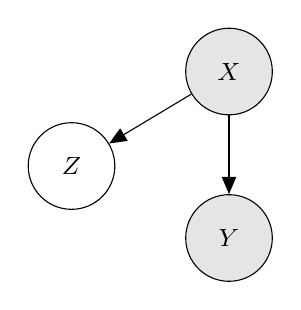
\begin{tikzpicture}[x=2cm, y=1.5cm]
 \node [io] (x) {$X$};
\node [neuron] at (-1, -0.8) (z) {$Z$};
\node [io, below=of x] (y) {$Y$};
\draw [->] (x) -- (z);
\draw [->] (x) -- (y);
\end{tikzpicture}
\caption{Graphical model of the information bottleneck}
\end{figure}

In the information bottleneck model, both the output and the representation depends solely on the input, that is we assume $p(z | x, y) = p(z|x)$. Most importantly, $Z$ is not part of the generative process of $Y$ as it would if $Z$ would be considered a latent variable of the model. In this case $Z$ is only there to ensure we learn a useful representation of $X$ that will help us to predict $Y$.

The factorisation theorem lets us express the joint distribution as:
$$ p(x, y, z) = p(x)\, p(y|x)\, p(z|x)$$

\subsection{Objective function}
In this section we will assume that the random variables are continuous. We define $p_\theta(z|x)$ as our stochastic encoding of the input where $\theta$ is the encoding parameter. The mutual information of the representation $Z$ and the target $Y$ can then be expressed as:

$$ I(Z, Y|\theta) = \int p(y, z|\theta) \log \frac{p(z, y|\theta)}{p(z|\theta)p(y)} dy\,dz $$

The objective of the information bottleneck method is to maximise $I(Z, Y|\theta)$ while constraining how much information is shared between $X$ and $Z$ such as to force $Z$ to "forget" $X$ and act as a minimal sufficient statistic of $X$ for predicting $Y$. The quantity we are constraining is therefore the mutual information of the input $X$ and its representation $Z$:

$$ I(X, Z|\theta) = \int p(x, z|\theta) \log \frac{p(x, z|\theta)}{p(x)p(z|\theta)} dy\,dz $$

So we want that $$I(X, Z) < I_c$$ where $I_c$ is the information constraint. This can be expressed using a Lagrange multiplier such as to write the whole objective function as:

$$ J_{IB}(\theta) = I(Z, Y|\theta) - \beta I(X, Z|\theta)$$


\subsection{Iterative Solution}
\begin{theorem}
The objective function has an exact formal solution when X, Y and Z are all discrete:
$$ p(z|x) = \frac{p(z)}{Z(x, \beta)} \exp\Big[-\beta \sum_y p(y|x) \log\frac{p(y|x)}{y|z}\Big] $$
\end{theorem}

 The proof can be found in \cite{tishby}. The expression $p(y|z)$ can be expressed as 
 
 \begin{align}
p(y|z) &= \sum_x p(y, x|z)  \\
	 & = \sum_x \frac{p(x ,y, z)}{p(z)} \\
	 &= \frac{1}{p(z)} \sum_x p(x) p(y|x) p (z|x) 
\label{eq:y_given_z}
\end{align}

And $p(z)$ can be expressed as a mixture:
 
  \begin{align}
p(z) &= \sum_x p(z, x)  \\
	 &= \sum_x p(x) p(z|x)
\label{eq:z_post}
\end{align}

In the formal solution, the encoder is present on both sides, Tishby et al. present a scheme to find a optimum by iteratively updating $p(z|x)$, $p(y|z)$ and $p(z)$.

\section{Monte Carlo Sampling}
\begin{theorem}[Law of large numbers]
If $X_i$ is a collection of independent identically distributed random variables with density $p(x)$, then
$$ \lim_{N \to \infty} \frac{1}{N} \sum_i f(X_i) = \int f(x) p(x) dx $$
\end{theorem}

In Monte Carlo sampling we use the law of large number to introduce an estimate  of the expectation:
Let $\theta = \mathbb{E}_{x \ sim p(x)}[f(X)]$

Then by the law of large number 

$$ \hat{\theta} =  \frac{1}{N} \sum_i f(X_i) $$ is an unbiased estimate of $\theta$.

\section{Recurrent Neural Networks}

\subsection{Architecture}
A neural network is a composition of linear and non-linear transformations organised in layers. It is a deterministic function of the input. The output of the neural network is given by:

$$ \hat{y} = f(x | W) = \sigma_L (W_L h_{L-1}(x)) $$

Where:
\begin{itemize}
\item $\hat{y}$ is the predicted output
\item $\sigma$ is a non-linear function
\item $W$ is the set of weights of the linear transformations
\item $L$ is the index of the output layer
\item $h_l$ are the hidden layers defined as:
  \begin{equation}
    \begin{cases}
          h_1(x) = \sigma_1(W_1 x)\\
          h_l(x) = \sigma_l (W_l h_{l-1}(x)) \quad \forall l \in \{2, L\}\\
    \end{cases}
  \end{equation}


\end{itemize}

\begin{figure}[H]
\centering
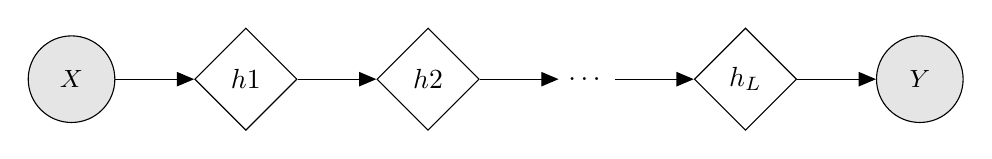
\begin{tikzpicture}[x=2cm, y=1.5cm]
 \node [io] (x) {$X$};
\node [deterministic, right=of x] (h1) {$h1$};
\node [deterministic, right=of h1] (h2) {$h2$};
\node [right=of h2](dots) {\ldots};
\node [deterministic, right=of dots] (hL) {$h_L$};
 \node [io, right=of hL] (y) {$Y$};
\draw [->] (x) -- (h1);
\draw [->] (h1) -- (h2);
\draw [->] (h2) -- (dots);
\draw [->] (dots) -- (hL);
\draw [->] (hL) -- (y);
\end{tikzpicture}
\caption{Graphical model of a neural network}
\end{figure}

In a recurrent neural network as introduced by Graves et al \cite{graves}, an input is given at each time step so the data is processed sequentially, this is especially useful to model language, music, stock prices, etc.

In that case the hidden states at each layer are a linear combination of the input and the previous hidden state such as to carry information from the past:
  \begin{equation}
    \begin{cases}
          h_1(x) = \sigma_1(W x) \\
          h_l(x_{1:l}) = \sigma_l (U h_{l-1}(x_{1:l-1}) + W x_l) \quad \forall l \in \{2, L\}\\
    \end{cases}
  \end{equation}

We use the same set of weights: U, W at each step since we are performing the same task with different inputs, this makes the parameter space much smaller.

When dealing with sequential data, there are several possible supervised learning problems:
\subsubsection{Many to many}
\begin{figure}[H]
\centering
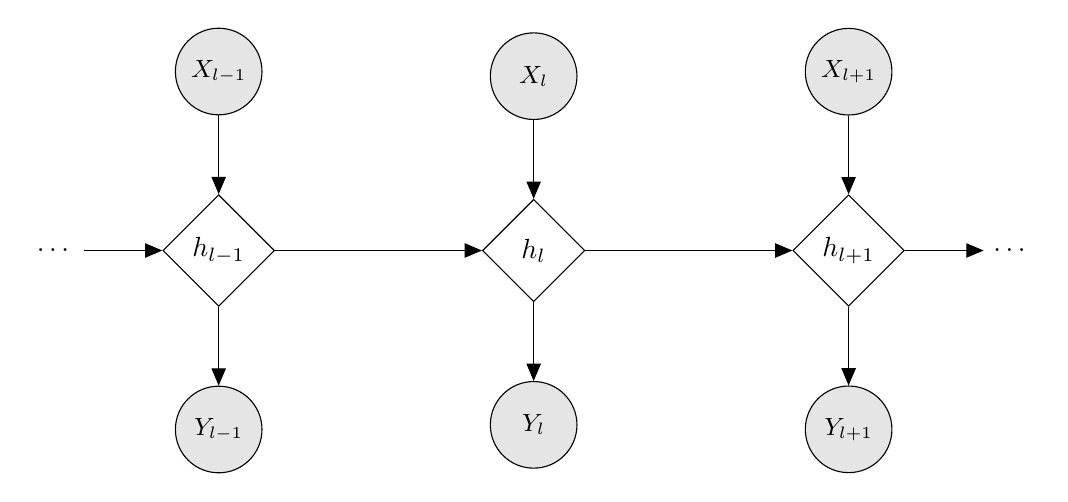
\begin{tikzpicture}[x=2cm, y=1.5cm]
\foreach \jlabel [count=\j, evaluate={\jj=int(\j-1); \jd=int(2 * \j);}]  in {l-1,  l, l+1}{
      \node [deterministic] at (\jd, 1) (h-\j) {$h_{\jlabel}$};
      \node [io, above=of h-\j] (x-\j) {$X_{\jlabel}$};
      \node [io, below=of h-\j] (y-\j) {$Y_{\jlabel}$};
      \draw [->] (x-\j) -- (h-\j);
      \draw [->] (h-\j) -- (y-\j);
      \ifnum\j>1
          \draw [->] (h-\jj.east) -- (h-\j.west);
      \fi
} 
\node [left=of h-1] (ldots){\ldots};
\node [right=of h-3] (rdots){\ldots};
\draw [->] (h-3) -- (rdots);
 \draw [->] (ldots) -- (h-1);
\end{tikzpicture}
\caption{Many to many recurrent neural network graphical model}
\end{figure}
In the many to many problem we try to predict the output at each time step based on previous inputs. For example, we try to predict the next pixel in an image, in that case the targets are the next inputs.

$$ \hat{y_l} = f(x_{1:l}|W, U, V) = V h_l(x_{1:l}|W,U)\quad \forall l \in \{1, L\}$$

\subsubsection{Many to one}
\begin{figure}[H]
\centering
\begin{tikzpicture}[x=2cm, y=1.5cm]
\foreach \jlabel [count=\j, evaluate={\jj=int(\j-1); \jd=int(2 * \j);}]  in {1,  2}{
      \node [deterministic] at (\jd, 1) (h-\j) {$h_{\jlabel}$};
      \node [io, above=of h-\j] (x-\j) {$X_{\jlabel}$};
      \draw [->] (x-\j) -- (h-\j);
      \ifnum\j>1
          \draw [->] (h-\jj.east) -- (h-\j.west);
      \fi
} 
\node [right=of h-2] (rdots){\ldots};
\draw [->] (h-2) -- (rdots);
\node [io, above=of h-3] (x-3) {$X_L$};
\node [deterministic, right=of rdots] (h-L) {$h_L$};
\draw [->] (rdots) -- (h-3);
\draw [->] (x-3) -- (h-3);
\node [io, below=of h-3] (y) {$Y$};
\draw [->] (h-L) -- (y);
\end{tikzpicture}
\caption{Many to one recurrent neural network graphical model }
\end{figure}

In the many to one problem, we try to predict the output after having seen a sequence. For example we try to predict the label of an image after sequentially processing all the pixels in the image.

$$ \hat{y} = f(x_{1:L}|W, U, V) = V h_L(x_{1:L}|W,U)$$

\subsubsection{Sequence to sequence}
\begin{figure}[H]
\centering
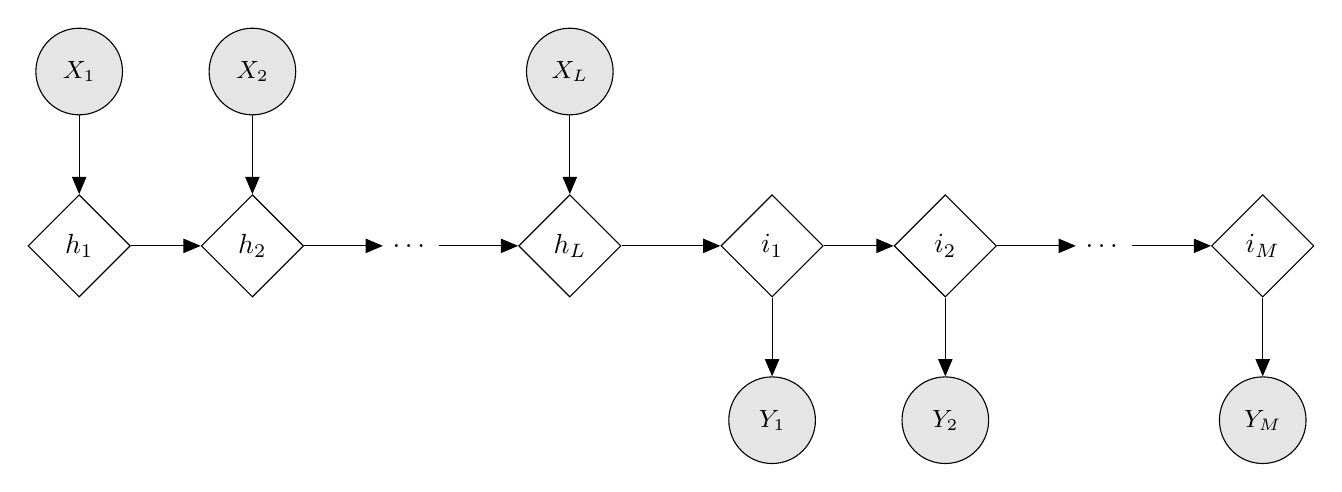
\begin{tikzpicture}[x=1.1cm, y=1.2cm]
\foreach \jlabel [count=\j, evaluate={\jj=int(\j-1); \jd=int(2 * \j);}]  in {1,  2}{
      \node [deterministic] at (\jd, 1) (h-\j) {$h_{\jlabel}$};
      \node [io, above=of h-\j] (x-\j) {$X_{\jlabel}$};
      \draw [->] (x-\j) -- (h-\j);
      \ifnum\j>1
          \draw [->] (h-\jj.east) -- (h-\j.west);
      \fi
} 
\node [right=of h-2] (rdots){\ldots};
\draw [->] (h-2) -- (rdots);
\node [deterministic, right=of rdots] (h-L) {$h_L$};
\node [io, above=of h-L] (x-L) {$X_L$};
\draw [->] (rdots) -- (h-L);
\draw [->] (x-L) -- (h-L);

\foreach \jlabel [count=\j, evaluate={\jj=int(\j-1); \jd=int(2 * \j);}]  in {1, 2}{
      \node [deterministic] at (8 + \jd, 1) (hpred-\j) {$i_{\jlabel}$};
      \node [io, below=of hpred-\j] (ypred-\j) {$Y_{\jlabel}$};
      \draw [->] (hpred-\j) -- (ypred-\j);
      \ifnum\j>1
          \draw [->] (hpred-\jj.east) -- (hpred-\j.west);
      \fi
} 
\draw [->] (h-L) -- (hpred-1);
\node [right=of hpred-2] (rdots){\ldots};
\draw [->] (hpred-2) -- (rdots);
\node [deterministic, right=of rdots] (hpred-M) {$i_M$};
\node [io, below=of hpred-M] (ypred-M) {$Y_M$};
\draw [->] (rdots) -- (hpred-M);
\draw [->] (hpred-M) -- (ypred-M);
\end{tikzpicture}
\caption{Sequence to sequence graphical model}
\end{figure}

Finally in the sequence to sequence problem we try to predict a sequence based on a partial sequence. For example we try to predict the 10 next pixels after having processed 100 pixels.

\begin{equation}
          \hat{y}_{m} = V i_{m} \quad \forall m \in \{1, M\}\\
\end{equation}

\subsection{Learning}
To learn in a neural network within a supervised learning setting, we introduce a loss function that we intend to minimise.

$$L = \sum_i L(y_i, \hat{y_i} = f(x_i|W))$$

Where $\{(x_i, y_i)\}$ is our training data. 

Since the gradient points in the direction of the steepest descent, the simplest way to learn is by taking the gradient of the loss with respect to each parameter and update their value at each iteration:

$$ W_{l, k+1} = W_{l, k} - \eta \nabla_{W_l} L(y, x, W) \quad \forall l \in \{1, L\}$$

Where $\eta$ is the learning rate.
 
To get the gradient with respect to each parameter $W_l$ we use the chain rule to backpropagate the gradient through the computational graph.
 
 \begin{align}
   \nabla_{W_l} L(y, x, W) &= \frac{\partial L}{\partial h_{L-1}} \nabla_{W_l} h_{L-1}\\
   &= \frac{\partial L}{\partial h_{L-1}} \frac{\partial h_{L-1}}{\partial h_{L-2}} \nabla_{W_l} h_{L-2}\\
   &...\\
   &= \frac{\partial L}{\partial h_{L-1}} \frac{\partial h_{L-1}}{\partial h_{L-2}} ... \frac{\partial h_l}{\partial W_l}
 \end{align}
 
In practice we use more complex optimisation method that take advantage of second-order derivatives. 
 
\subsection{Vanishing Gradients}
In the recurrent neural network setting, our network can be very deep as every input adds a layer. As a consequence gradients will either vanish or explode depending of the initialisation of the weights, this will prevent learning the optimal weights.

\subsection{Gated Recurrent Unit}
To overcome the vanishing or exploding gradient problem, different architecture were proposed including the Gated Recurrent Unit \cite{gru}. Instead of taking $h_l = \sigma(U h_l + W x_l)$ they introduce a gate mechanism that allows a better control of the information that flows through the graph.

The operation performed are the following:
\begin{align}
z_t &= \sigma_g(W_{z} x_t + U_{z} h_{t-1} + b_z) \\
r_t &= \sigma_g(W_{r} x_t + U_{r} h_{t-1} + b_r) \\
h_t &=  z_t \circ h_{t-1} + (1-z_t) \circ \sigma_h(W_{h} x_t + U_{h} (r_t \circ h_{t-1}) + b_h)
\end{align}
Where:
\begin{itemize}
 \item $z_t$ is the update gate that defines how much of the previous memory we keep
 \item $r_t$ is the reset gate that determines how to combine the new input with the previous memory state
\item  $\sigma_g$ is the sigmoid function
\item $\sigma_h$ is a hyperbolic tangent
\end{itemize}
%------------------------------------------------------------------------------------------------
\chapter{Further Considerations}
\section{Mutual Information and Maximum Likelihood in Supervised Setting}

We consider the simplest graphical model in a supervised learning setting:

\begin{center}
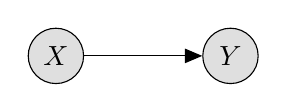
\begin{tikzpicture}
    \node[obs] (x) {$X$} ; 
    \node[obs, right=1.5cm of x] (y) {$Y$} ; 
    \draw [->] (x) -- (y) ; 
\end{tikzpicture}
\end{center}

We would like to check that maximising the mutual information between X and Y is equivalent to maximum likelihood:

\begin{align}
E_{X, Y}[\log p(y|x)] &= \int p(x, y)\log p(y| x)\, dx\,dy\\ 
&= - H(Y | X)\
\end{align}


\begin{align}
I(X, Y) &= H(Y) - H(Y|X)
\end{align}

So if we consider the entropy of the labels fixed, maximising the mutual information is indeed equivalent to maximum likelihood.

\section{Mutual Information Maximisation in Stochastic Feed-forward Network}

We consider a graphical model in a supervised learning setting:

\begin{figure}[H]
  \centering
  \tikz{ %
    \node[obs] (x) {$X$} ; %
    \node[latent, right=of x] (z) {$Z$} ; %
    \node[obs, right=of z] (y) {$Y$} ; %
    \edge {x} {z} ; %
    \edge {z} {y} ; %
  }
\end{figure}

Where X is our observed data and Y our labels. Z is a stochastic representation of our data.

\subsection{Maximum Likelihood}

We try to maximise the likelihood $\log p(y|x)$

\subsubsection{Naive approach}

The simplest way to do this would be to sample directly from the likelihood:

\begin{align}
 p(y|x) &= \int p(y, z|x) dz \\
 &= \int p(y|z) p(z|x) dz \\
 &= E_{Z | X}[p(y|z)] 
\end{align}

For example:
$$ p(y|z) = S(y | Wz + b) $$ were S is the softmax function.
And:
$$ p(z|x) \sim \mathcal{N}(z | f^\mu(x), f^\Sigma(x))$$ where $f^\mu$ and $f^\Sigma$ are multi-layer perceptrons.

We can approximate
\begin{align}
 p(y|x) &\approx \frac{1}{M} \sum^M_{m=1} p(y | z^{(m)}) 
\end{align}

Where $ z^{(m)} \sim p(z|x) $

However this might lead to a high variance because we can't be sure that our draw from $p(z | x)$ will contribute significantly to our estimate $p(y |x)$.

\subsubsection{Stochastic Gradient Variational Bayes}

To prevent this, we use a variational lower bound on the log likelihood:
\begin{align}
 \log p(y|x) &= \log(\int p(y, z|x) dz) \\
 & =  \log(\int q(z) \frac{p(y, z|x)}{q(z)}) \\
 & \geq \int q(z) \log \frac{p(y, z|x)}{q(z)}
\end{align}

Using Jensen's inequality.

\begin{align}
 \log p(y|x) & \geq \int q(z) \log \frac{p(z|x) p(y| z)}{q(z)} \\
  &= \int q(z) \log \frac{p(z|x)}{q(z)}  + \int q(z) \log p(y|z) \\
  &= E_q[p(y|z)] - KL[q(z) || p(z|x)]\\
  &\approx  \frac{1}{M} \sum^M_{m=1} p(y | z^{(m)}) - KL[q(z) || p(z|x)]
\end{align}
Where $ z^{(m)} \sim q(z)$ and assuming the KL divergence can be computed analytically.

So we try to maximise the expected value of decoder given z sampled from a distribution parametrised by the encoder while minimising the KL divergence between $q(z)$ and $p(z|x)$.

\subsection{Maximum Mutual Information}

We would like to compare this result to the maximisation of the  mutual information between Z and Y:

\begin{align}
I(Z, Y) &= \int p(y, z) \log \frac{p(z, y)}{p(z)p(y)} dy\,dz\\
& = \int p(y, z) \log \frac{p(y|z)}{p(y)} dy\,dz\\
&= \int p(y, z) \log p(y|z) dy\,dz - H(y) 
\end{align}
We ignore the entropy of the labels as it can't be maximised. We get:
\begin{align}
I(Z, Y) &= \int p(x, y, z) \log p(y| z) dx\,dy\,dz\\
&= \int p(z | x, y) p(x, y) \log p(y | z) dx\,dy\,dz
\end{align}
We can approximate the joint distribution of the data and the labels by:
$$ p(x, y) \approx \frac{1}{N}\sum_n \delta_{x_n}(x) \delta_{y_n}(y)$$
So we get:
$$ I(Z, Y) \approx \frac{1}{N} \int p(z | x^{(n)}, y^{(n}) \log p(y^{(n)} | z) $$

As we can see this is not equivalent to the maximum likelihood. In particular we have no way to easily get the posterior over z.

%------------------------------------------------------------------------------------------------
\chapter{Model}
\section{Deep Variational Information Bottleneck}

In the previous section a solution to the information bottleneck problem was presented when X, Y and Z are all discrete. However in the general case there won't be a formal solution or an iterative method to find the parametric encoder. Alemi at al. in \cite{vib} introduce a variational approach to the information bottleneck. They use variational inference to provide a lower bound to the information bottleneck objective. This allow us to use stochastic gradient ascent to find an optimum of the lower bound and to parametrise the encoder with a neural network which can handle a broad range of data.

\subsection{Variational Lower Bound}

The equation \ref{eq:y_given_z} is not tractable in the continuous case. Using $q(y|z)$ as a variational approximation to $p(y|z)$ we can find a lower bound to the mutual information of $Y$ and $Z$ as proposed in Barber et al. \cite{barber}.

\begin{lemma}
A lower bound to the mutual information of $Y$ and $Z$ is:
$$ I(Z, Y) \geq  \int p(x)\, p(y|x)\, p(z|x) \log q(y|z) dy\, dz\, dx + H(Y)$$
\end{lemma}

\begin{proof}
Given that the KL divergence is necessarily positive we have 

$$ KL[p(y|z)|q(y|z)] \geq 0$$
Therefore 
$$ \int p(y|z) \log \frac{p(y|z)}{q(y_z)} dy \geq 0 $$
$$ \Rightarrow \int p(y|z) \log p(y|z) dy \geq \int p(y|z) \log q(y|z) dy$$
$$ \Rightarrow \frac{1}{p(z)} \int p(y, z) \log p(y|z) dy \geq  \frac{1}{p(z)} \int p(y, z) \log q(y|z) dy$$
$$\Rightarrow  \int p(y, z) \log p(y|z) dy \geq  \int p(y, z) \log q(y|z) dy$$
$$\Rightarrow  \int p(y, z) \log p(y|z) dy\, dz\geq  \int p(y, z) \log q(y|z) dy\, dz$$
$$\Rightarrow  \int p(y, z) \log p(y|z) dy\, dz - \int p(y, z) \log p(y) dy\, dz\geq  \int p(y, z) \log q(y|z) dy\, dz - \int p(y, z) \log p(y) dy\, dz$$

 \begin{align}
 \Rightarrow I(Z, Y) &\geq  \int p(y, z) \log q(y|z) dy\, dz + H(Y)\\
	  &=  \int p(x, y, z) \log q(y|z) dy\, dz\, dx + H(Y)\\
	  &=  \int p(x) p(y|x) p(z|x) \log q(y|z) dy\, dz\, dx + H(Y)
\end{align}
\end{proof}
If $q(z|y) = p(z|y)$, the bound is exact. 

Note that since the entropy of the label is a constant, it will be ignored in our objective function.

We also approximate the marginal on $Z$ $p(z)$ given in equation \ref{eq:z_post} by $r(z)$ which gives us the second part of the objective function.

\begin{lemma}
An upper bound to the mutual information of $X$ and $Z$ is:
$$ I(Z, Y) \geq  \int p(x)p(y|x)p(z|x) \log \frac{p(z|x)}{r(z)}dx\, dy\, dz$$
\end{lemma}

\begin{proof}
$$ KL[p(z)|r(z)] \geq 0$$
Therefore 
$$ \int p(z) \log \frac{p(z)}{r(z)} dz \geq 0 $$
$$ \Rightarrow \int p(z) \log p(z) dz\geq \int r(z) \log p(z) dz$$
$$ \Rightarrow \int p(z, x) \log p(z) dx\, dz \geq \int r(z, x) \log p(z) dx\, dz$$
$$ \Rightarrow -\int p(z, x) \log p(z) dx\, dz\leq - \int r(z, x) \log p(z) dx\, dz$$
$$ \Rightarrow \int p(z, x) \log p(z|x)dx\, dz -\int p(z, x) \log p(z) dx\, dz\leq  \int p(z, x) \log p(z|x)dx\, dz - \int r(z, x) \log p(z) dx\, dz $$
 \begin{align}
I(X, Z) & \leq  \int p(z, x) \log \frac{p(z|x)}{r(z)} dx\, dz\\
   	  & =  \int p(x, y, z) \log \frac{p(z|x)}{r(z)}dx\, dy\, dz \\
   	  & = \int p(x)p(y|x)p(z|x) \log \frac{p(z|x)}{r(z)}dx\, dy\, dz \\
\end{align}
\end{proof}

\begin{theorem}
A lower bound to the information bottleneck objective function can be written as:
 \begin{align}
J(\theta) &= I(Z, Y|\theta) - \beta I(X, Z|\theta)\\
	      &\geq \int p(x) p(y|x) p(z|x) \log q(y|z) dy\, dz\, dx - \beta   \int p(x)p(y|x)p(z|x) \log \frac{p(z|x)}{r(z)} dx\, dy\, dz
\end{align}
\end{theorem}

One possibility to to find an optimum to this problem would be to update iteratively the model parameter $\theta$ from $p_\theta(z|x)$  and the variational parameters $\phi$ and $\psi$ from $q_\phi(y|z)$ and $r_\psi(z)$ in a procedure similar to the expectation maximisation algorithm for the maximum likelihood. However in this case we will use stochastic gradient descent to optimise the bound.

\subsection{Empirical joint distribution}
Since X and Y are known during training, we can use the empirical data distribution $p(x, y) \approx \frac{1}{N}\sum_n\delta_{x_n}(x)\delta_{y_n}(y)$ to approximate the lower bound:

 \begin{align}
L & = \int p(x, y) p(z|x) \log q(y|z) dx\, dy\, dz - \beta \int p(x, y) p(z|x) \log \frac{p(z|x)}{r(z)}dx\, dy\, dz  \\
   & = \int \frac{1}{N}\sum_n\delta_{x_n}(x)\delta_{y_n}(y) p(z|x) \log q(y|z) dy\, dz\, dx \\ 
   & \quad - \beta  \int \frac{1}{N}\sum_n\delta_{x_n}(x)\delta_{y_n}(y) p(z|x) \log \frac{p(z|x)}{r(z)}dx\, dy\, dz \\
   & = \frac{1}{N}\sum_n \Big[ \int \delta_{x_n}(x)\delta_{y_n}(y) p(z|x) \log q(y|z) dy\, dz\, dx \\
   & \quad - \beta   \int \delta_{x_n}(x)\delta_{y_n}(y) p(z|x) \log \frac{p(z|x)}{r(z)}dx\, dy\, dz \Big] \\
   & = \frac{1}{N}\sum_n \Big[ \int p(z|x_n) \log q(y_n|z_n) - \beta   p(z|x_n) \log \frac{p(z|x_n)}{r(z)} dz \Big] \label{eq:lower}
\end{align}


\subsection{Reparametrisation Trick}
The main issue with the lower bound as it is given in \ref{eq:lower} is that that gradient with respect to the encoding parameter is not well defined. Indeed the gradient can't be propagated through $Z$ as it is a stochastic layer.

\begin{figure}[H]
    \centering
    \begin{minipage}{0.45\textwidth}
        \centering
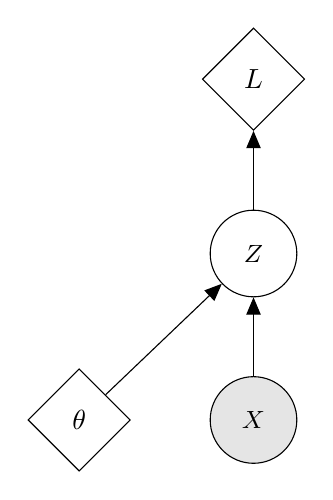
\begin{tikzpicture}[x=2cm, y=1.5cm]
 \node [neuron] (z) {$Z$};
\node [io, below=of z] (x) {$X$};
\node [deterministic, left=of x] (theta) {$\theta$};
\node [deterministic, above=of z] (l) {$L$};
\draw [->] (x) -- (z);
\draw [->] (theta) -- (z);
\draw [->] (z) -- (l);
\end{tikzpicture}
        \caption{first figure}
    \end{minipage}\hfill
    \begin{minipage}{0.45\textwidth}
        \centering
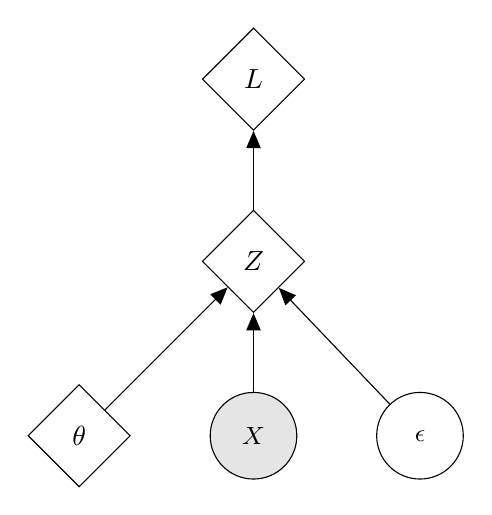
\begin{tikzpicture}[x=2cm, y=1.5cm]
 \node [deterministic] (z) {$Z$};
\node [io, below=of z] (x) {$X$};
\node [deterministic, left=of x] (theta) {$\theta$};
\node [deterministic, above=of z] (l) {$L$};
\node [neuron, right=of x] (eps) {$\epsilon$};
\draw [->] (x) -- (z);
\draw [->] (theta) -- (z);
\draw [->] (z) -- (l);
\draw [->] (eps) -- (z);
\end{tikzpicture}
        \caption{second figure}
    \end{minipage}
\end{figure}

To solve this issue, we use the reparametrisation trick also called pathwise estimator  from Kingma \& Welling \cite{kingma} and write $z$ as a deterministic function of the model parameter $\theta$ and a random variable $\epsilon$: $z = f(\theta(x), \epsilon)$ and
$$p(z) = p(\epsilon) \Big|\frac{d\epsilon}{dz} \Big| \Rightarrow |p(\epsilon) d\epsilon| = |p(z|x) dz|$$
The gradient can then be propagated back to the input and the parameters through the deterministic node $Z$:
\begin{align}
\nabla_\theta \int p_\theta(z|x) g(z) dz &= \nabla_\theta \int p(\epsilon) g(f(\theta(x), \epsilon))\\
&= \int p(\epsilon) \nabla_\theta g(f(\theta(x), \epsilon))\\
&= \mathbb{E}_{p(\epsilon)}[\nabla_\theta g(f(\theta(x), \epsilon))]
\end{align}

We can therefore rewrite the objective function as:

 \begin{align}
L   &= \frac{1}{N}\sum_n  \mathbb{E}_{\epsilon \sim p(\epsilon)}\Big[  \log q(y_n|f(x_n, \epsilon)) - \beta  \log \frac{p(f(x_n, \epsilon)|x_n)}{r(f(x_n, \epsilon))}\Big]  \label{eq:lower2}
\end{align}

Note that if the the KL divergence can be calculated analytically as it is the case if both distribution are gaussian we can write more simply:

 $$ L = \frac{1}{N}  \sum_{n=1}^{N} \mathbb{E}_{\epsilon \sim p(\epsilon)}[\log q(y_{n} |f(x_{n}, \epsilon))] - \beta KL[p(Z|x_{n}), r(Z)]$$

To turn this into a convex problem, the obective function we try to minimise is:

 $$ J_{VIB} = \frac{1}{N}  \sum_{n=1}^{N} \mathbb{E}_{\epsilon \sim p(\epsilon)}[- \log q(y_{n} |f(x_{n}, \epsilon))] + \beta KL[p(Z|x_{n}), r(Z)]$$


\section{Application to Sequential Data}

We apply the variational information bottleneck method to find a good representation of a sequence rather than a single input. This is useful to avoid overfitting on the training data when predicting future outputs. We will use recurrent neural networks to combine the inputs and pass the hidden layer of the network through an information bottleneck to get a robust representation of the sequence. As we have seen there are different supervised learning problem for sequential data we will see how to apply the variational information bottleneck in each setting.

\subsection{Many to many}
\begin{figure}[H]
\centering
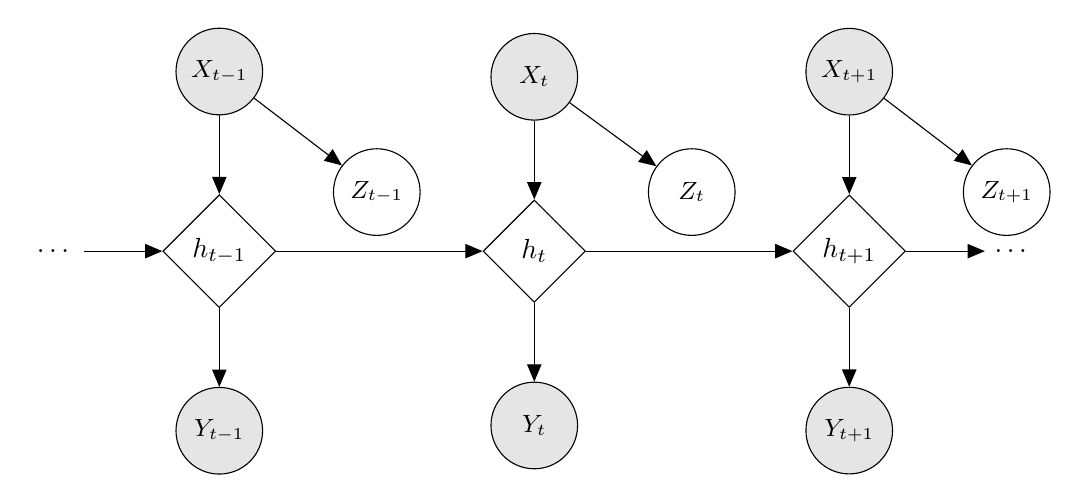
\begin{tikzpicture}[x=2cm, y=1.5cm]
\foreach \jlabel [count=\j, evaluate={\jj=int(\j-1); \jd=int(2 * \j);}]  in {t-1,  t, t+1}{
      \node [deterministic] at (\jd, 1) (h-\j) {$h_{\jlabel}$};
       \node [neuron] at (\jd + 1, 1.5) (z-\j) {$Z_{\jlabel}$};
      \node [io, above=of h-\j] (x-\j) {$X_{\jlabel}$};
      \node [io, below=of h-\j] (y-\j) {$Y_{\jlabel}$};
      \draw [->] (x-\j) -- (h-\j);
      \draw [->] (x-\j) -- (z-\j);
      \draw [->] (h-\j) -- (y-\j);
      \ifnum\j>1
          \draw [->] (h-\jj.east) -- (h-\j.west);
      \fi
} 
\node [left=of h-1](ldots) {\ldots};
\node [right=of h-3](rdots) {\ldots};
\draw [->] (ldots) -- (h-1);
\draw [->] (h-3) -- (rdots);
\end{tikzpicture}
\caption{Graphical model of many to many variational information bottleneck}
\end{figure}

In the many to many problem we try to find at each time step a representation $Z_t$ that is maximally compressive of each input $X_t$ and maximally predictive about future outputs. The objective function can therefore be written as:

$$ J_{IB} = \sum_t I(Z_t, Y_{t}) - \beta I(X_{t}, Z_t)$$
 
 The problem with this setting is that the representation $Z_t$ does not contain information about the past, therefore they won't be good predictor of the outputs. One way to solve this would be to have $Z_t$ depend on all previous inputs. However in that case the $Z_t$ won't be independent and therefore we wouldn't be able to decompose the objective function as we did.
 
\subsection{Many to one}

\begin{figure}[H]
\centering
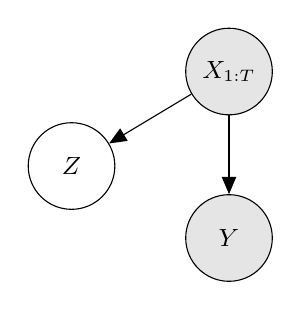
\begin{tikzpicture}[x=2cm, y=1.5cm]
 \node [io] (x) {$X_{1:T}$};
\node [neuron] at (-1, -0.8) (z) {$Z$};
\node [io, below=of x] (y) {$Y$};
\draw [->] (x) -- (z);
\draw [->] (x) -- (y);
\end{tikzpicture}
\caption{Graphical model of many to one variational information bottleneck}
\end{figure}

The many to one problem is similar to the original supervised problem. Indeed we can consider the whole sequence as a random variable and apply the information bottleneck on this. When implementing this we will use the output of a recurrent neural network and pass it through the information bottleneck to get a good representation of the sequence. 

\begin{figure}[H]
\centering
\begin{tikzpicture}[x=2cm, y=1.5cm]
\foreach \jlabel [count=\j, evaluate={\jj=int(\j-1); \jd=int(2 * \j);}]  in {1,  2}{
      \node [deterministic] at (\jd, 1) (h-\j) {$h_{\jlabel}$};
      \node [io, above=of h-\j] (x-\j) {$X_{\jlabel}$};
      \draw [->] (x-\j) -- (h-\j);
      \ifnum\j>1
          \draw [->] (h-\jj.east) -- (h-\j.west);
      \fi
} 
\node [right=of h-2] (rdots){\ldots};
\draw [->] (h-2) -- (rdots);
\node [io, above=of h-3] (x-3) {$X_T$};
\node [deterministic, right=of rdots] (h-L) {$h_T$};
\draw [->] (rdots) -- (h-3);
\draw [->] (x-3) -- (h-3);
\node [neuron] at (7, 3.5) (z) {$Z$};
\draw [->] (x-1.north) -- (z);
\draw [->] (x-2.north) -- (z);
\draw [->] (x-3.north) -- (z);
\node [io, right=of h-L] (y) {$Y$};
\draw [->] (h-L) -- (y);
\end{tikzpicture}
\caption{Graphical model of many to one variational information bottleneck }
\end{figure}

If we draw the graphical model as a sequence we note that the hidden states represented are the hidden states of the generative model rather than the hidden state of the encoder. 

The information bottleneck objective is then:
$$ J_{IB} = I(Z, Y) - \beta I(X_{1:T}, Z)$$
Whose lower bound objective under the variational approximation becomes:
 $$ J_{VIB} = \frac{1}{N}  \sum_{n=1}^{N} \mathbb{E}_{\epsilon \sim p(\epsilon)}[- \log q(y_{n} |f(x_{1:T, n}, \epsilon))] + \beta KL[p(Z|x_{1:T, n}), r(Z)]$$

\subsection{Sequence to Sequence}
Sequence to sequence problems have first been used in the context of recurrent neural network by Sutskever \cite{s2s}.


\begin{figure}[H]
\centering
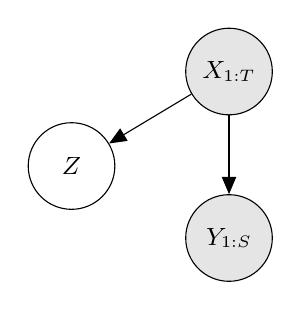
\begin{tikzpicture}[x=2cm, y=1.5cm]
 \node [io] (x) {$X_{1:T}$};
\node [neuron] at (-1, -0.8) (z) {$Z$};
\node [io, below=of x] (y) {$Y_{1:S}$};
\draw [->] (x) -- (z);
\draw [->] (x) -- (y);
\end{tikzpicture}
\caption{Sequence to sequence variational information bottleneck graphical model}
\end{figure}


\begin{figure}[H]
\centering
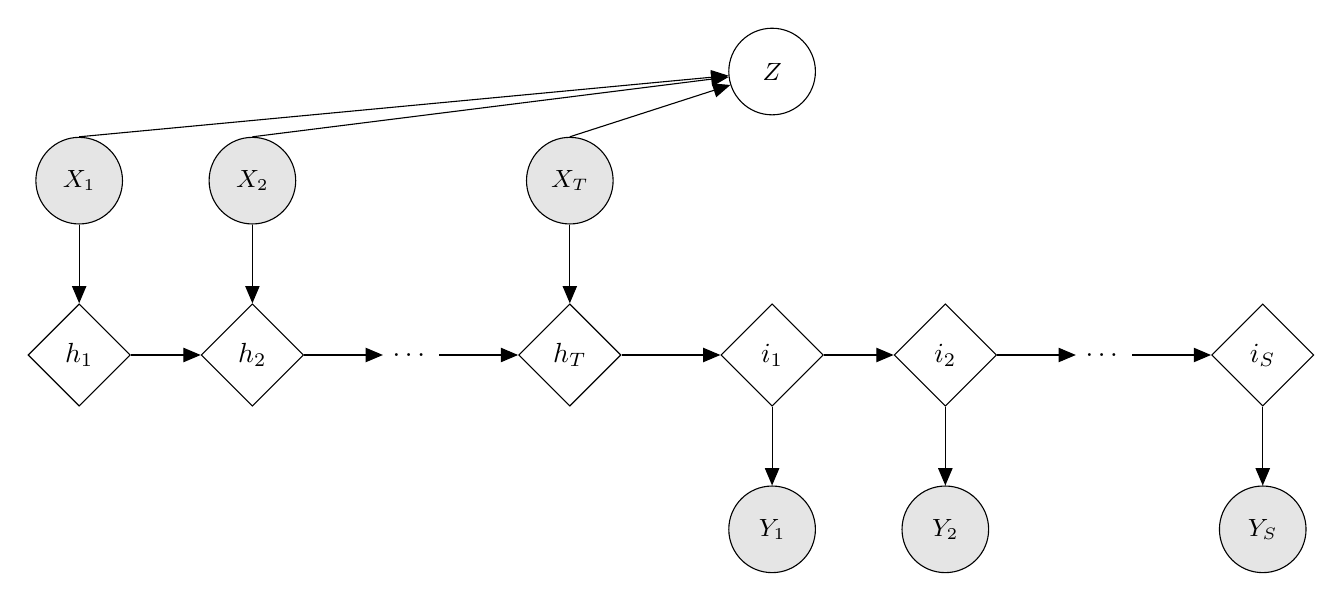
\begin{tikzpicture}[x=1.1cm, y=1.2cm]
\foreach \jlabel [count=\j, evaluate={\jj=int(\j-1); \jd=int(2 * \j);}]  in {1,  2}{
      \node [deterministic] at (\jd, 1) (h-\j) {$h_{\jlabel}$};
      \node [io, above=of h-\j] (x-\j) {$X_{\jlabel}$};
      \draw [->] (x-\j) -- (h-\j);
      \ifnum\j>1
          \draw [->] (h-\jj.east) -- (h-\j.west);
      \fi
} 
\node [right=of h-2] (rdots){\ldots};
\draw [->] (h-2) -- (rdots);
\node [deterministic, right=of rdots] (h-L) {$h_T$};
\node [io, above=of h-L] (x-L) {$X_T$};
\draw [->] (rdots) -- (h-L);
\draw [->] (x-L) -- (h-L);

\foreach \jlabel [count=\j, evaluate={\jj=int(\j-1); \jd=int(2 * \j);}]  in {1, 2}{
      \node [deterministic] at (8 + \jd, 1) (hpred-\j) {$i_{\jlabel}$};
      \node [io, below=of hpred-\j] (ypred-\j) {$Y_{\jlabel}$};
      \draw [->] (hpred-\j) -- (ypred-\j);
      \ifnum\j>1
          \draw [->] (hpred-\jj.east) -- (hpred-\j.west);
      \fi
} 
\draw [->] (h-L) -- (hpred-1);
\node [right=of hpred-2] (rdots){\ldots};
\draw [->] (hpred-2) -- (rdots);
\node [deterministic, right=of rdots] (hpred-M) {$i_S$};
\node [io, below=of hpred-M] (ypred-M) {$Y_S$};
\draw [->] (rdots) -- (hpred-M);
\draw [->] (hpred-M) -- (ypred-M);
\node [neuron] at (10, 4) (z) {$Z$};
\draw [->] (x-1.north) -- (z);
\draw [->] (x-2.north) -- (z);
\draw [->] (x-L.north) -- (z);
\end{tikzpicture}
\caption{Sequence to sequence variational information bottleneck graphical model}
\end{figure}

The information bottleneck objective is then:
$$ J_{IB} = I(Z, Y_{1:S}) - \beta I(X_{1:T}, Z)$$
Whose lower bound objective under the variational approximation becomes:
 $$ J_{VIB} = \frac{1}{N}  \sum_{n=1}^{N} \mathbb{E}_{\epsilon \sim p(\epsilon)}[- \log q(y_{1:S, n} |f(x_{1:T, n}, \epsilon))] + \beta KL[p(Z|x_{1:T, n}), r(Z)]$$

\chapter{Implementation}
\section{Stochastic encoder $p(z|x)$}
Like in \cite{vib} we choose our encoder to be a gaussian whose mean and variance will be given by the output of a neural network:
$$ p(z|x) \sim \mathcal{N}(z | f^\mu(x), f^\Sigma(x))$$ where $f^\mu$ and $f^\Sigma$ are neural networks / multi-layer perceptrons. The last layer of the perceptron is processed by two sets of linear weights, the first gives the mean and we apply a softplus to the second which gives the diagonal standard deviation terms.

\section{Reparametrisation trick}
Since the encoder is a gaussian we can use  $z = f(x, \epsilon) =  \mu(x) + \Sigma(x) \epsilon$ for the reparametrisation trick where $\epsilon \sim \mathcal{N}(0, I)$. 
 
\section{Decoder $q(y|z)$}
For the variational approximation of $p(y|z)$ we use a simple logistic regression:

$$ q(z|x) = \mathcal{S}(y|f(z))$$ where $f(z)$ is a linear transformation. and $\mathcal{S} is the softmax function.$

\section{Marginal $r(z)$}

As an approximation to the marginal we use $r(z) \sim \mathcal{N}(0, 1)$

To improve the expressiveness of the prior distribution on the latent, we allow its parameters to be learned. 

$$p(z) \sim \mathcal{N}(\mu_p, \Sigma_p)$$

The KL divergence between 2 gaussians with diagonal variance:

\begin{align}
KL(\mathcal{N}_q, \mathcal{N}_p) &= \frac{1}{2}(Tr(\Sigma_p^{-1}\Sigma_q) + (\mu_p - \mu_q)^T\Sigma_p^{-1}(\mu_p - \mu_q) - k + \log\frac{|\Sigma_p|}{|\Sigma_q|})\\
&= \frac{1}{2}(\sum_i \frac{\Sigma_{q, ii}}{\Sigma_{p, ii}} + \sum_i \frac{(\mu_{p_i} - \mu_{q, i})^2}{\Sigma_{p, ii}} - k + \log\frac{\prod \Sigma_{p, ii}}{\prod \Sigma_{q, ii}})\\
&= \frac{1}{2}(\sum_i[ \log \Sigma_{p, ii} - \log \Sigma_{q, ii} - 1 + \frac{\Sigma_{q, ii}}{\Sigma_{p, ii}} + \frac{(\mu_{p_i} - \mu_{q, i})^2}{\Sigma_{p, ii}}]
\end{align}

Beforehand we had assumed a standard normal prior which gave:
\begin{align}
KL(\mathcal{N}_q, \mathcal{N}_0) &= \sum_i[ -\log \Sigma_{q, ii} - 1 + \Sigma_{q, ii}+ \mu_{q, i}^2]
\end{align}

\section{Expectation}

In the lower bound we have to take an expectation with respect $p(\epsilon)$. To do so we take S Monte Carlo samples 
 $$ \mathbb{E}_{\epsilon \sim p(\epsilon)}[- \log q(y_{n} |f(x_{n}, \epsilon))] \approx \frac{1}{S}\sum_s - \log q(y_{n} |f(x_{n}, \epsilon_s)) $$
 
 We used S = 1 or S = 12.


%------------------------------------------------------------------------------------------------
\chapter{Results}
TODO

%------------------------------------------------------------------------------------------------
\chapter{Conclusion}
TODO

\appendix
%------------------------------------------------------------------------------------------------
\chapter{First Appendix}

\begin{thebibliography}{9} 
\bibitem{barber}
David Barber and Felix Agakov
\textit{The IM Algorithm : A variational approach to Information Maximization}
NIPS 2004
\bibitem{tishby} 
N. Tishby, F.C. Pereira, and W. Biale.
\textit{The information bottleneck method}.
37th annual Allerton Conference on Communication, Control, and Computing, pp. 368-377, 1999.
\bibitem{vib} 
A. A. Alemi, I. Fischer, J. V. Dillon, and K. Murphy
\textit{Deep variational information bottleneck}.
 arXiv:1612.00410, 2016.
 \bibitem{kingma} 
 Diederik P Kingma and Max Welling.
 \textit{Auto-encoding variational Bayes.}
  ICLR, 2014
 \bibitem{gru} 
 Junyoung Chung, Caglar Gulcehre, KyungHyun Cho, Yoshua Bengio.
 \textit{Empirical Evaluation of Gated Recurrent Neural Networks on Sequence Modeling.}
  NIPS, 2014
 \bibitem{graves}
 Graves, Alex.
 \textit{Generating sequences with recurrent neural networks.}
 CoRR, abs/1308.0850, 2013
\bibitem{s2s}
Ilya Sutskever, Oriol Vinyals and Quoc V. Le
\textit{Sequence to Sequence Learning with Neural Networks}
NIPS 2014

\end{thebibliography}
\end{document}
